% ============================================================
%  Codificadores de visión para Modelos Visión-Lenguaje (VLMs)
%  Clase de posgrado — Beamer (metropolis), compilar con pdflatex
% ============================================================
\documentclass[aspectratio=169,10pt]{beamer}
\usetheme{metropolis}

\usepackage[T1]{fontenc}
\usepackage[utf8]{inputenc}
\usepackage{amsmath,amssymb,bm}
\usepackage{booktabs,multirow,array}
\usepackage{xcolor}
\usepackage{listings}

% ---------- Paleta ----------
\definecolor{cVis}{HTML}{1F77B4}   % visión
\definecolor{cTxt}{HTML}{D62728}   % texto
\definecolor{cProj}{HTML}{2CA02C}  % proyector
\definecolor{cLLM}{HTML}{9467BD}   % LLM
\definecolor{cConv}{HTML}{FF7F0E}  % convolución
\definecolor{cAtt}{HTML}{17BECF}   % atención
\definecolor{cGray}{HTML}{7F7F7F}
\setbeamercolor{alerted text}{fg=cTxt}

% ---------- Español sin babel ----------
\renewcommand{\figurename}{Figura}
\renewcommand{\tablename}{Tabla}
\newcommand{\ie}{i.\,e.}
\newcommand{\eg}{p.\,ej.}

% ---------- Código ----------
\lstset{
  language=Python, basicstyle=\ttfamily\scriptsize, keywordstyle=\color{cVis}\bfseries,
  commentstyle=\color{cGray}\itshape, stringstyle=\color{cTxt}, showstringspaces=false,
  frame=single, rulecolor=\color{black!20}, backgroundcolor=\color{black!3},
  literate={á}{{\'a}}1 {é}{{\'e}}1 {í}{{\'i}}1 {ó}{{\'o}}1 {ú}{{\'u}}1 {ñ}{{\~n}}1
}

% ---------- Recuadros ----------
\newcommand{\refbox}[1]{\begin{flushright}\vspace{-2mm}{\scriptsize\color{cGray}#1}\end{flushright}}

\title{LLMs \& VLMs course}
\subtitle{Codificadores de visión para VLMs}
\author{Juan Irving Vasquez}
\date{\today}
\institute{Instituto Politécnico Nacional (IPN)}
\titlegraphic{
\includegraphics[height=1.2cm]{ipn-cidetec.png}\hspace{0.1cm}
\includegraphics[height=1.2cm]{escudoESCOM}}

\begin{document}

% ============================================================
\maketitle

\frame{
	\frametitle{Contents}
	\tableofcontents
}

\AtBeginSection[] { \begin{frame} \frametitle{Roadmap} \tableofcontents[currentsection] \end{frame} }




% ============================================================
\section{Contexto: el codificador de visión dentro de un VLM}
% ============================================================

\begin{frame}{Anatomía de un VLM}
  \centering
  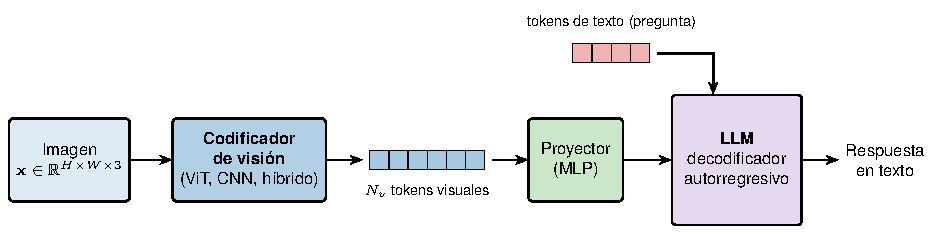
\includegraphics[width=.95\textwidth]{Figuras/anatomia_llava}

  \vspace{4mm}
  \begin{columns}[T]
    \column{.5\textwidth}
    \small
    \begin{itemize}
      \item Tres piezas: \textcolor{cVis}{\textbf{encoder}}, \textcolor{cProj}{\textbf{proyector}}, \textcolor{cLLM}{\textbf{LLM}}.
      \item El encoder suele venir \alert{preentrenado con CLIP} y alineado con el lenguaje.
      \item LLaVA usa features de la \emph{penúltima} capa de un CLIP ViT-L/14.
    \end{itemize}
    \column{.5\textwidth}
    \small
    \begin{itemize}
      \item Otras arquitecturas: cross-attention (Flamingo/Frozen), \emph{early fusion} con codebook (Chameleon), sin encoder (Fuyu, EVE).
      \item Según FastVLM, las variantes sin encoder todavía \alert{rinden menos} que las que usan un encoder preentrenado.
    \end{itemize}
  \end{columns}
  \refbox{Liu et al., LLaVA, NeurIPS 2023 (arXiv:2304.08485); Liu et al., LLaVA-1.5, CVPR 2024 (arXiv:2310.03744)}
\end{frame}

\begin{frame}{Evolución de las arquitecturas VLM: ¿dónde vive el encoder?}
  \centering
  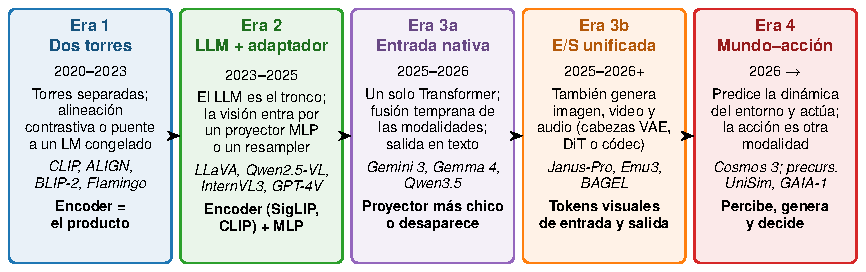
\includegraphics[width=\textwidth]{Figuras/evolucion_vlm}
  \vspace{1mm}
  \begin{itemize}\small
    \item En todas las eras se repiten los mismos ingredientes: un \alert{tokenizador o encoder visual}, el lado de lenguaje y un módulo de alineación. Cambia \alert{dónde ocurre la fusión} y qué produce el modelo.
    \item Esta clase se centra en las eras 1 (CLIP) y 2 (LLaVA, COMM, FastVLM), donde el encoder es un módulo identificable y sustituible.
  \end{itemize}
  \refbox{Li et al., Survey (2026), §2–§3.4 y Fig.~2}
\end{frame}

\begin{frame}{¿Qué le pedimos a un codificador de visión para VLMs?}
  \begin{columns}[T]
    \column{.55\textwidth}
    \begin{enumerate}
      \item \textbf{Semántica alineada con lenguaje} $\Rightarrow$ preentrenamiento imagen–texto (CLIP, SigLIP, \dots).
      \item \textbf{Alta resolución}: crucial para OCR, documentos, gráficas (TextVQA, DocVQA).
      \item \textbf{Pocos tokens visuales} $N_v$: cada token cuesta en el \emph{prefill} del LLM.
      \item \textbf{Baja latencia del encoder}, sobre todo en dispositivo.
    \end{enumerate}
    \column{.45\textwidth}
    \begin{block}{Métrica clave: \emph{Time-To-First-Token}}
      \[
        \text{TTFT} \;=\; \underbrace{T_{\text{enc}}(r)}_{\text{encoder}} \;+\; \underbrace{T_{\text{prefill}}\big(N_v(r)+N_t\big)}_{\text{LLM}}
      \]
      con $r$ la resolución de entrada.
    \end{block}
    \small Tensión central de la clase: \alert{subir $r$ mejora la precisión pero aumenta $T_{\text{enc}}$ y $N_v$}.
  \end{columns}
  \refbox{Vasu et al., FastVLM (2025), §1 y §3.2.1}
\end{frame}

% ============================================================
\section{Vision Transformer (ViT)}
% ============================================================

\begin{frame}{La idea: una imagen vale 16$\times$16 palabras}
  \centering
  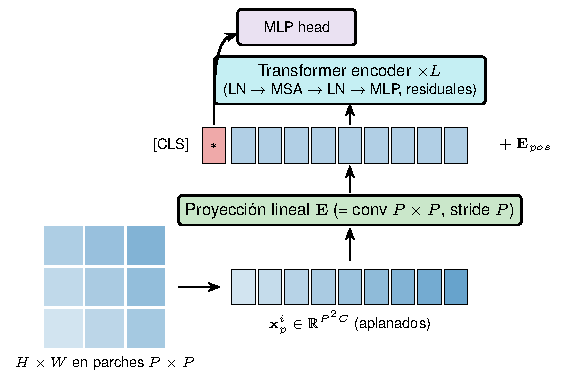
\includegraphics[height=.7\textheight]{Figuras/vit_parches}
  \begin{itemize}\small
    \item Transformer estándar de NLP, \alert{casi sin modificaciones}; único sesgo de imagen: el corte en parches (y el ajuste de resolución en fine-tuning).
  \end{itemize}
  \refbox{Dosovitskiy et al., ViT (2021), Fig.~1 y §3.1}
\end{frame}

\begin{frame}{Formulación}
  Sea $N = HW/P^2$ el número de parches, $D$ la dimensión latente:
  \begin{align*}
    \mathbf{z}_0 &= [\,\mathbf{x}_{\text{class}};\ \mathbf{x}_p^1\mathbf{E};\ \mathbf{x}_p^2\mathbf{E};\ \cdots;\ \mathbf{x}_p^N\mathbf{E}\,] + \mathbf{E}_{pos}, &
    \mathbf{E}&\in\mathbb{R}^{(P^2C)\times D},\ \mathbf{E}_{pos}\in\mathbb{R}^{(N+1)\times D} \\
    \mathbf{z}'_\ell &= \mathrm{MSA}(\mathrm{LN}(\mathbf{z}_{\ell-1})) + \mathbf{z}_{\ell-1}, & \ell&=1,\dots,L\\
    \mathbf{z}_\ell &= \mathrm{MLP}(\mathrm{LN}(\mathbf{z}'_{\ell})) + \mathbf{z}'_{\ell}, & \ell&=1,\dots,L\\
    \mathbf{y} &= \mathrm{LN}(\mathbf{z}_L^0)
  \end{align*}
  \vspace{-2mm}
  \begin{columns}[T]
    \column{.5\textwidth}
    \begin{block}{Autoatención multi-cabeza}
      \small
      $\mathrm{SA}(\mathbf{z}) = \mathrm{softmax}\!\big(\mathbf{q}\mathbf{k}^\top/\sqrt{D_h}\big)\,\mathbf{v}$,\\
      $[\mathbf{q},\mathbf{k},\mathbf{v}]=\mathbf{z}\,\mathbf{U}_{qkv}$; $k$ cabezas con $D_h=D/k$.
    \end{block}
    \column{.5\textwidth}
    \begin{block}{Costo por capa}
      \small
      Atención: $\mathcal{O}(N^2 D)$ \quad MLP: $\mathcal{O}(N D^2)$\\
      $\Rightarrow$ \alert{cuadrático en $N$}, y $N$ crece \alert{cuadráticamente} con el lado de la imagen.
    \end{block}
  \end{columns}
  \refbox{ViT, Ecs.~(1)–(4) y Apéndice A}
\end{frame}

\begin{frame}{Variantes y nomenclatura}
  \begin{columns}[c]
    \column{.52\textwidth}
    \centering
    \begin{tabular}{lcccc r}
      \toprule
      Modelo & Capas & $D$ & MLP & Cabezas & Params \\
      \midrule
      ViT-Base  & 12 & 768  & 3072 & 12 & 86M \\
      ViT-Large & 24 & 1024 & 4096 & 16 & 307M \\
      ViT-Huge  & 32 & 1280 & 5120 & 16 & 632M \\
      \bottomrule
    \end{tabular}

    \vspace{3mm}
    \small \textbf{ViT-L/14} = Large con parches de $14\times14$.\\ Menor $P$ $\Rightarrow$ más tokens $\Rightarrow$ más caro.
    \column{.48\textwidth}
    \centering
    \small Tokens de un ViT con $P=14$:\\[1mm]
    \begin{tabular}{rr}
      \toprule
      Resolución & $N=(r/14)^2$ \\
      \midrule
      $224^2$ & 256 \\
      $336^2$ & \textbf{576} \ (LLaVA-1.5) \\
      $672^2$ & 2\,304 \\
      $1008^2$ & 5\,184 \\
      \bottomrule
    \end{tabular}

    \vspace{2mm}
    \small Duplicar el lado $\Rightarrow$ $4\times$ tokens $\Rightarrow$ $\sim16\times$ costo de atención.
  \end{columns}
  \refbox{ViT, Tabla 1}
\end{frame}

\begin{frame}{Sesgo inductivo vs. escala de datos}
  \begin{columns}[T]
    \column{.5\textwidth}
    \textbf{Lo que ViT \emph{no} trae de fábrica}
    \begin{itemize}\small
      \item Localidad, estructura 2D de vecindarios, equivarianza a traslaciones: en una CNN están en \emph{cada} capa.
      \item En ViT sólo las MLP son locales; la autoatención es global.
      \item Las relaciones espaciales entre parches se \alert{aprenden desde cero}.
    \end{itemize}
    \column{.5\textwidth}
    \textbf{Hallazgo empírico}
    \begin{itemize}\small
      \item Entrenado sólo en ImageNet-1k, ViT queda \alert{por debajo} de ResNets de tamaño similar.
      \item Con ImageNet-21k y JFT-300M: ``\emph{large scale training trumps inductive bias}''.
      \item ViT-H/14 (JFT-300M): \textbf{88.55\%} top-1 en ImageNet, con menos cómputo de preentrenamiento que BiT/Noisy Student.
    \end{itemize}
  \end{columns}
  \vspace{2mm}
  \begin{exampleblock}{Lección para VLMs}
    Por eso el encoder de un VLM casi nunca se entrena desde cero: se \alert{hereda} de un preentrenamiento masivo (supervisado, o mejor aún, imagen–texto como CLIP).
  \end{exampleblock}
  \refbox{ViT, §3.1 (Inductive bias), §4.2 y §4.3}
\end{frame}

\begin{frame}{Cambiar de resolución: interpolación de los embeddings de posición}
  \begin{columns}[c]
    \column{.55\textwidth}
    \begin{itemize}\small
      \item Fine-tuning a mayor resolución con el mismo $P$ $\Rightarrow$ secuencia más larga.
      \item El Transformer acepta cualquier longitud, pero $\mathbf{E}_{pos}$ pierde sentido.
      \item Solución de ViT: \alert{interpolación 2D} de $\mathbf{E}_{pos}$ según la posición en la imagen original.
      \item Es uno de los dos únicos puntos donde se inyecta a mano la estructura 2D.
    \end{itemize}
    \vspace{2mm}
    \small\textbf{Relevancia hoy:} así se adaptan los CLIP-ViT de $224$ a $336$ (o más) en VLMs; pero el costo sigue creciendo como $\mathcal{O}(N^2)$.
    \column{.45\textwidth}
    \centering
    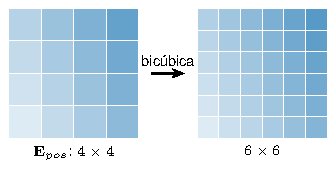
\includegraphics[width=\linewidth]{Figuras/vit_pos_interp}
  \end{columns}
  \refbox{ViT, §3.2 (Fine-tuning and higher resolution)}
\end{frame}

% ============================================================
\section{CLIP y más allá: ¿qué encoder y qué capa?}
% ============================================================

\begin{frame}{Motivación}
  \begin{columns}[T]
    \column{.5\textwidth}
    \textbf{Problema de la supervisión clásica}
    \begin{itemize}\small
      \item Conjunto \alert{fijo} de categorías (\eg 1000 de ImageNet).
      \item Cada concepto nuevo requiere más datos etiquetados.
    \end{itemize}
    \vspace{2mm}
    \textbf{Propuesta}
    \begin{itemize}\small
      \item Aprender directamente de \alert{texto crudo} sobre imágenes.
      \item Tarea proxy: \emph{¿qué texto va con qué imagen?}
      \item El lenguaje natural sirve para \alert{referirse} a conceptos nuevos $\Rightarrow$ transferencia \emph{zero-shot}.
    \end{itemize}
    \column{.5\textwidth}
    \begin{block}{Datos: WIT (WebImageText)}
      \small
      \begin{itemize}
        \item \textbf{400 millones} de pares (imagen, texto) de Internet.
        \item Construido a partir de $\sim$500k consultas; hasta $\sim$20k pares por consulta para balancear.
        \item Número total de palabras similar al de WebText (GPT-2).
      \end{itemize}
    \end{block}
  \end{columns}
  \refbox{Radford et al., CLIP (2021), §1 y §2.2}
\end{frame}

\begin{frame}{Arquitectura de doble torre y objetivo contrastivo}
  \begin{columns}[c]
    \column{.58\textwidth}
    \centering
    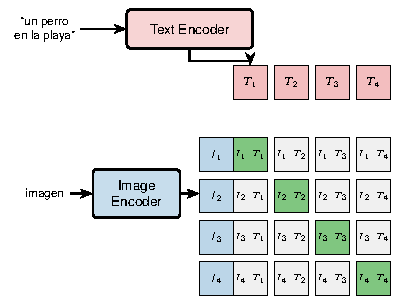
\includegraphics[width=\linewidth]{Figuras/clip_doble_torre}
    \column{.42\textwidth}
    \small
    \begin{itemize}
      \item Batch de $n$ pares $\Rightarrow$ matriz de similitudes coseno $n\times n$.
      \item \textcolor{cProj}{\textbf{Diagonal}}: $n$ pares reales (positivos).
      \item Fuera de la diagonal: $n^2-n$ negativos.
      \item Proyecciones \alert{lineales} a un espacio común; embeddings normalizados $\ell_2$.
      \item Ambos encoders se entrenan \alert{desde cero}.
    \end{itemize}
  \end{columns}
  \refbox{CLIP, Fig.~1 y §2.3}
\end{frame}

\begin{frame}[fragile]{Pérdida contrastiva simétrica (InfoNCE)}
  \begin{columns}[T]
    \column{.48\textwidth}
    Con $s_{ij} = \langle \mathbf{I}_i, \mathbf{T}_j\rangle$ (embeddings normalizados) y temperatura $\tau$:
    \[
      \mathcal{L}_{I\to T} = -\frac{1}{n}\sum_{i=1}^{n}\log\frac{e^{s_{ii}/\tau}}{\sum_{j=1}^{n} e^{s_{ij}/\tau}}
    \]
    \[
      \mathcal{L}_{T\to I} = -\frac{1}{n}\sum_{j=1}^{n}\log\frac{e^{s_{jj}/\tau}}{\sum_{i=1}^{n} e^{s_{ij}/\tau}}
    \]
    \[
      \mathcal{L} = \tfrac{1}{2}\big(\mathcal{L}_{I\to T}+\mathcal{L}_{T\to I}\big)
    \]
    \small $\tau$ es \alert{aprendida} (log-parametrizada), inicializada en $0.07$ y recortada para que el factor $1/\tau$ no pase de 100.
    \column{.52\textwidth}
\begin{lstlisting}
# I[n,h,w,c], T[n,l]: minibatch alineado
I_f = image_encoder(I)          # [n, d_i]
T_f = text_encoder(T)           # [n, d_t]

# embedding multimodal conjunto [n, d_e]
I_e = l2_normalize(I_f @ W_i, axis=1)
T_e = l2_normalize(T_f @ W_t, axis=1)

# similitudes coseno escaladas [n, n]
logits = (I_e @ T_e.T) * np.exp(t)

# pérdida simétrica
labels = np.arange(n)
loss_i = cross_entropy(logits, labels, axis=0)
loss_t = cross_entropy(logits, labels, axis=1)
loss   = (loss_i + loss_t) / 2
\end{lstlisting}
  \end{columns}
  \refbox{CLIP, Fig.~3 y §2.5}
\end{frame}

\begin{frame}{¿Por qué contrastivo y no generativo?}
  \begin{columns}[c]
    \column{.5\textwidth}
    \centering
    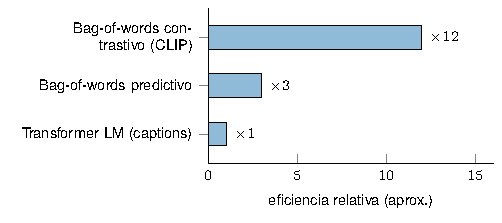
\includegraphics[width=\linewidth]{Figuras/clip_eficiencia}
    \column{.5\textwidth}
    \small
    \begin{itemize}
      \item Predecir el texto \alert{exacto} de una imagen es muy difícil: hay muchas descripciones válidas.
      \item Predecir una bolsa de palabras: $\sim3\times$ más eficiente en zero-shot ImageNet.
      \item Pasar a objetivo contrastivo: \alert{otro $\sim4\times$}.
      \item Idea: basta con identificar \emph{qué texto completo} va con \emph{qué imagen}.
    \end{itemize}
  \end{columns}
  \refbox{CLIP, Fig.~2 y §2.3 (valores de la figura redondeados)}
\end{frame}

\begin{frame}{Encoders y entrenamiento}
  \begin{columns}[T]
    \column{.5\textwidth}
    \textbf{Encoder de imagen}
    \begin{itemize}\small
      \item \textbf{ResNet} modificada (ResNet-D, blur pooling) con \alert{attention pooling}: una capa de atención con la query condicionada al promedio global de la imagen.
      \item \textbf{ViT} con una LayerNorm extra sobre parches + posiciones antes del Transformer.
      \item 5 ResNets (RN50 $\to$ RN50x64) y 3 ViTs (B/32, B/16, L/14).
    \end{itemize}
    \textbf{Encoder de texto}
    \begin{itemize}\small
      \item Transformer de 63M parámetros, 12 capas, ancho 512, 8 cabezas; BPE de 49\,152 tokens; máximo 76 tokens.
      \item Representación: activación de la capa final en el token \texttt{[EOS]}.
    \end{itemize}
    \column{.5\textwidth}
    \textbf{Receta de entrenamiento}
    \begin{itemize}\small
      \item 32 épocas, Adam con weight decay desacoplado, cosine schedule.
      \item Minibatch de \alert{32\,768} (muchos negativos).
      \item RN50x64: 18 días en 592 V100.
      \item ViT-L/14: 12 días en 256 V100.
      \item \textbf{ViT-L/14@336px}: una época extra a 336 px; es el mejor modelo.
    \end{itemize}
    \vspace{1mm}
    \begin{alertblock}{Dato conectado con VLMs}
      \small CLIP ViT-L/14@336px es el encoder de LLaVA-1.5: \textbf{576 tokens} visuales.
    \end{alertblock}
  \end{columns}
  \refbox{CLIP, §2.4 y §2.5}
\end{frame}

\begin{frame}{Transferencia zero-shot}
  \begin{columns}[c]
    \column{.52\textwidth}
    \centering
    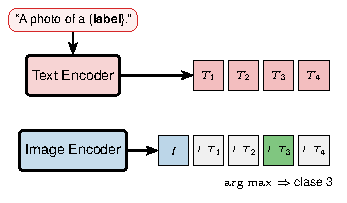
\includegraphics[width=\linewidth]{Figuras/clip_zeroshot}
    \[
      p(y=k\mid \mathbf{x}) = \frac{\exp(\langle \mathbf{I},\mathbf{T}_k\rangle/\tau)}{\sum_{j}\exp(\langle \mathbf{I},\mathbf{T}_j\rangle/\tau)}
    \]
    \column{.48\textwidth}
    \small
    \begin{itemize}
      \item El encoder de texto actúa como \alert{hiper-red}: genera los pesos de un clasificador lineal a partir de los nombres de clase.
      \item \textbf{Ingeniería de prompts}: ``A photo of a \{label\}.'' mejora ImageNet en 1.3\% frente al nombre solo.
      \item \textbf{Ensamble} de 80 prompts: junto con la ingeniería, casi \alert{+5 puntos} en promedio.
      \item Zero-shot ImageNet: de 11.5\% (Visual N-Grams) a \alert{76.2\%}, al nivel de una ResNet-50 supervisada, sin usar ninguna de sus 1.28M imágenes etiquetadas.
    \end{itemize}
  \end{columns}
  \refbox{CLIP, §3.1}
\end{frame}

\begin{frame}{Por qué CLIP domina los VLMs\dots\ y dónde se queda corto}
  \begin{columns}[T]
    \column{.48\textwidth}
    \textbf{Fortalezas}
    \begin{itemize}\small
      \item Más \alert{robusto a cambios de distribución} (ImageNet-V2, Sketch, R, A, ObjectNet) que supervisados con igual precisión.
      \item Sus features ya ``\alert{hablan el idioma}'' del texto: al VLM le basta un proyector simple.
      \item Vocabulario visual abierto; escala bien con datos.
    \end{itemize}
    \small Descendientes en VLMs: SigLIP (pérdida sigmoide), EVA-CLIP, DFN-CLIP, InternViT, MobileCLIP\dots
    \column{.52\textwidth}
    \textbf{Límites (según CLIP)}
    \begin{itemize}\small
      \item Tareas finas (modelos de autos), abstractas (contar) o fuera de distribución (MNIST); sesgos de datos web.
    \end{itemize}
    \textbf{Límites como rama visual (según COMM)}
    \begin{itemize}\small
      \item Supervisión \alert{global} (captions): pierde detalle a nivel píxel (color, posición) $\Rightarrow$ peor \emph{grounding}, más alucinación.
      \item Se usan sólo capas \alert{profundas} (penúltima), que codifican lo global.
      \item Desbalance ViT-L ($\sim$300M) vs.\ Vicuna 7B/13B: por el ``\alert{efecto cubeta}'', el encoder es la tabla más corta.
    \end{itemize}
  \end{columns}
  \refbox{CLIP, §3.3 y §6; Jiang et al., COMM (2024), §1 y §3}
\end{frame}

\begin{frame}{¿Qué paradigma de preentrenamiento sirve como rama visual?}
  \small
  COMM: 4 encoders ViT-L + Vicuna-7B (tipo Shikra), evaluados en \emph{grounding} (REC), alucinación (POPE), regiones (REG), VQA y MME.

  \centering\footnotesize
  \begin{tabular}{>{\raggedright\arraybackslash}p{2.6cm} >{\raggedright\arraybackslash}p{1.9cm} >{\raggedright\arraybackslash}p{2.6cm} >{\raggedright\arraybackslash}p{5.4cm}}
    \toprule
    Paradigma & Ejemplo & Señal de entrenamiento & Resultado como rama visual \\
    \midrule
    Contrastivo imagen–texto & CLIP, EVA-CLIP & captions (global) & Buena semántica y fácil de alinear; detalle fino limitado en capas profundas \\
    \addlinespace
    Autosupervisado sólo imagen & DINOv2 & imágenes curadas, sin texto & Con un \alert{MLP} para alinear, \alert{supera a CLIP en grounding}; semántica aceptable \\
    \addlinespace
    Imagen enmascarada (MIM) & MAE & reconstruir píxeles & REC aceptable, pero cae mucho en POPE y REG: \alert{poca semántica} \\
    \addlinespace
    Supervisado & DeiT & etiquetas de ImageNet & El peor: espacio muy especializado, \alert{difícil de alinear} con el texto \\
    \bottomrule
  \end{tabular}
  \vspace{1mm}
  \raggedright\footnotesize
  La survey agrupa los encoders en dos familias: preentrenados con \textbf{pares imagen–texto} (CLIP, BLIP) y en \textbf{ImageNet o similares}, supervisados o autosupervisados (ResNet, ViT). Ambas superan a un encoder entrenado desde cero.
  \refbox{COMM, §3 y Fig.~2; Survey, §3.1}
\end{frame}

\begin{frame}{¿Qué capa? COMM: fusión multinivel de CLIP y DINOv2}
  \begin{columns}[T]
    \column{.5\textwidth}
    \footnotesize
    \begin{itemize}
      \item \textbf{CLIP}: capas \alert{superficiales} $\to$ detalle local, mejor REC; profundas $\to$ semántica global.
      \item \textbf{DINOv2}: las capas profundas ya son finas; las superficiales \alert{no} aportan semántica.
      \item \textbf{COMM}: todas las capas de CLIP + capas 19–24 de DINOv2, con Linear+LN y pesos aprendidos:
    \end{itemize}
    \scriptsize
    \[
      \bar{\mathbf{v}}_1=\sum_{i=1}^{24}\alpha_i\,\mathrm{Lin}(\mathrm{LN}(\mathbf{v}_1^i)),\quad
      \bar{\mathbf{v}}_2=\sum_{j=19}^{24}\beta_j\,\mathrm{Lin}(\mathrm{LN}(\mathbf{v}_2^j))
    \]
    \[
      \hat{\mathbf{v}}=\mathrm{Linear}\big([\,\bar{\mathbf{v}}_1;\ \mathrm{MLP}(\bar{\mathbf{v}}_2)\,]\big)\ \to\ \text{LLM}
    \]
    \footnotesize Encoders \alert{congelados}, $336^2$; se entrenan LLM, alineación y fusión.
    \column{.5\textwidth}
    \centering\scriptsize
    \begin{tabular}{lrrrr}
      \toprule
      Rama visual & REC & POPE & MME-P & VQAv2 \\
      \midrule
      CLIP (capa 23) & 47.3 & 82.3 & 1107.8 & 68.8 \\
      DINOv2 & 54.8 & 78.3 & 930.5 & 63.1 \\
      CLIP + MFM & 70.0 & 83.4 & 1164.4 & 69.5 \\
      DINOv2 + MFM & \textbf{72.8} & 83.3 & 1086.8 & 68.0 \\
      \textbf{COMM} & \textbf{72.8} & \textbf{83.6} & \textbf{1234.9} & \textbf{70.1} \\
      \bottomrule
    \end{tabular}

    \vspace{1mm}
    {\tiny Promedios en la configuración de análisis (entrenamiento corto).}

    \vspace{2mm}
    \small RefCOCO val (modelo completo, 7B): \textbf{COMM 91.7} vs. Qwen-VL 89.4 vs. Shikra 87.0.

    \vspace{2mm}
    \begin{exampleblock}{Idea clave}
      \small No basta la última capa de CLIP: \alert{combinar niveles} y \alert{combinar encoders} complementarios mejora la percepción fina.
    \end{exampleblock}
  \end{columns}
  \refbox{COMM, §3–§4, Ec.~(1), Tablas 1 y 2}
\end{frame}

% ============================================================
\section{El problema de la resolución}
% ============================================================

\begin{frame}{Tokens visuales vs. resolución}
  \begin{columns}[c]
    \column{.56\textwidth}
    \centering
    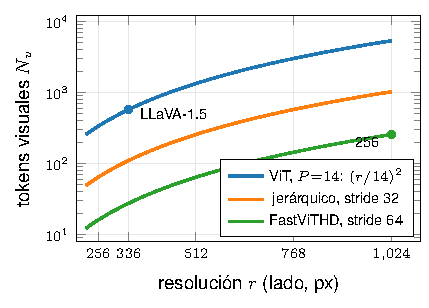
\includegraphics[width=\linewidth]{Figuras/tokens_resolucion}
    \column{.44\textwidth}
    \small
    \textbf{Dos costos que suben con $r$:}
    \begin{enumerate}
      \item $T_{\text{enc}}$: el encoder procesa más píxeles; en ViT, atención $\mathcal{O}(N^2)$.
      \item $T_{\text{prefill}}$: el LLM recibe $N_v$ tokens extra.
    \end{enumerate}
    \vspace{2mm}
    A $1024^2$: ViT-L/14 $\approx$ 5\,350 tokens; FastViTHD produce \alert{256}.
  \end{columns}
\end{frame}

\begin{frame}{Estrategias para tener alta resolución sin pagar de más}
  \footnotesize
  \begin{tabular}{>{\raggedright\arraybackslash}p{3.2cm} >{\raggedright\arraybackslash}p{5.2cm} >{\raggedright\arraybackslash}p{4.8cm}}
    \toprule
    Estrategia & Idea & Costo / limitación \\
    \midrule
    \textbf{Tiling} (AnyRes, S$^2$, Sphinx) & Partir la imagen en mosaicos a la resolución nativa del encoder & Varias pasadas del encoder; tokens se multiplican \\
    \addlinespace
    \textbf{Poda / fusión de tokens} (PruMerge, VisionZip, FastV, SparseVLM) & Descartar o fusionar tokens poco informativos & Diseño adicional; el encoder sigue siendo caro \\
    \addlinespace
    \textbf{Remuestreadores} (Perceiver, Q-Former) & $M$ queries aprendidas atienden a todos los tokens & Módulo extra, puede perder detalle fino \\
    \addlinespace
    \textbf{Backbone jerárquico} (ConvNeXt, FastViT, FasterViT) & Reducir resolución espacial \alert{dentro} del encoder & Hay que diseñarlo para que sea rápido y preentrenarlo con CLIP \\
    \bottomrule
  \end{tabular}
  \vspace{3mm}

  \normalsize FastVLM apuesta por la última: \alert{escalar sólo la resolución de entrada}, sin poda ni remuestreadores.
  \refbox{FastVLM, §1–§2}
\end{frame}

\begin{frame}{Isotrópico vs. jerárquico}
  \centering
  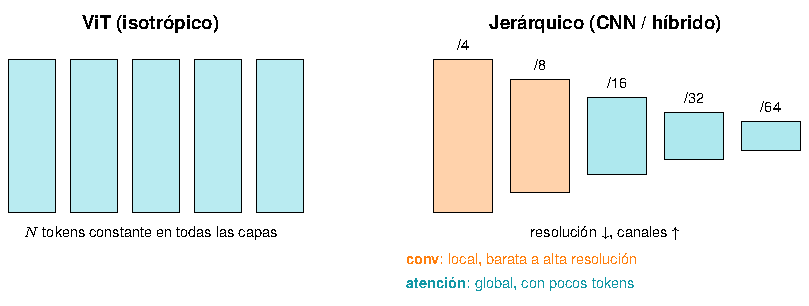
\includegraphics[width=\textwidth]{Figuras/isotropico_jerarquico}
  \vspace{3mm}
  \begin{itemize}\small
    \item Un encoder jerárquico \alert{reduce tokens de manera natural}: no hace falta podar después.
    \item Las convoluciones escalan \alert{linealmente} en píxeles y llevan el sesgo inductivo que le falta a ViT.
    \item La atención en las etapas finales refina tokens de alta calidad para el LLM.
  \end{itemize}
\end{frame}

% ============================================================
\section{FasterViT: atención jerárquica}
% ============================================================

\begin{frame}{Principio de diseño: pensar en el hardware}
  \begin{columns}[T]
    \column{.5\textwidth}
    \textbf{Etapas tempranas} (alta resolución, pocos canales, \eg $112\times112\times64$)
    \begin{itemize}\small
      \item \alert{Limitadas por memoria} (memory-bound).
      \item Conviene usar \alert{convoluciones densas}, no depthwise.
      \item Evitar operaciones no matriciales (normalización, SE, etc.).
    \end{itemize}
    \column{.5\textwidth}
    \textbf{Etapas tardías} (\eg $14\times14$, muchos canales)
    \begin{itemize}\small
      \item \alert{Limitadas por cómputo} (math-bound).
      \item Hay margen para LayerNorm, atención multi-cabeza, etc., con poco efecto en throughput.
    \end{itemize}
  \end{columns}
  \vspace{4mm}
  \centering
  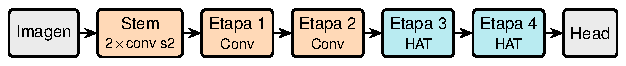
\includegraphics[width=\textwidth]{Figuras/fastervit_etapas}

  \small Bloque conv: $\hat{\mathbf{x}}=\mathrm{GELU}(\mathrm{BN}(\mathrm{Conv}_{3\times3}(\mathbf{x})))$,\ \ $\mathbf{x}\leftarrow\mathrm{BN}(\mathrm{Conv}_{3\times3}(\hat{\mathbf{x}}))+\mathbf{x}$; downsampling: LN 2D + conv $3\times3$ stride 2.
  \refbox{Hatamizadeh et al., FasterViT (2024), §3.1–§3.3}
\end{frame}

\begin{frame}{Hierarchical Attention (HAT): carrier tokens}
  \begin{columns}[c]
    \column{.42\textwidth}
    \centering
    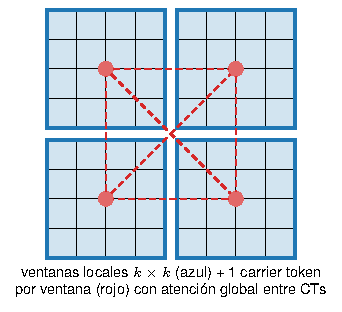
\includegraphics[width=\linewidth]{Figuras/hat_carrier_tokens}
    \column{.58\textwidth}
    \small
    \begin{enumerate}
      \item Partir el mapa $\mathbf{x}\in\mathbb{R}^{H\times W\times d}$ en $n^2=H^2/k^2$ ventanas:\ $\hat{\mathbf{x}}_l=\mathrm{Split}_{k\times k}(\mathbf{x})$.
      \item Inicializar \alert{carrier tokens} (CT) por ventana:\\ $\hat{\mathbf{x}}_{ct}=\mathrm{AvgPool}(\mathrm{Conv}_{3\times3}(\mathbf{x}))$, \ $L$ CTs por ventana, $L\ll k$.
      \item Atención \alert{global entre CTs}:\\ $\hat{\mathbf{x}}_{ct}\!\leftarrow\!\hat{\mathbf{x}}_{ct}+\gamma_1\mathrm{MHSA}(\mathrm{LN}(\hat{\mathbf{x}}_{ct}))$, luego MLP.
      \item Concatenar cada ventana con \alert{sus} CTs y aplicar atención local:\\ $\hat{\mathbf{x}}_w=\mathrm{Concat}(\hat{\mathbf{x}}_l,\hat{\mathbf{x}}_{ct,l})$.
      \item Separar y repetir; al final de la etapa:\\ $\mathbf{x}=\mathrm{Upsample}(\hat{\mathbf{x}}_{ct,l})+\mathrm{Merge}(\hat{\mathbf{x}}_l)$.
    \end{enumerate}
    \vspace{1mm}
    Posición: sesgo absoluto 2D vía MLP + sesgo relativo log-espaciado (SwinV2) $\Rightarrow$ \alert{flexible a cualquier resolución}.
  \end{columns}
  \refbox{FasterViT, Ecs.~(2)–(8), Figs.~2 y 4}
\end{frame}

\begin{frame}{Complejidad: ¿por qué HAT escala casi lineal?}
  Mapa de $H\times H$ (\ie $N=H^2$ tokens), dimensión $d$, ventana $k$, $L$ CTs por ventana:
  \vspace{2mm}
  \begin{center}
  \begin{tabular}{l c l}
    \toprule
    Atención & Complejidad & Contexto global \\
    \midrule
    Completa (ViT) & $\mathcal{O}(H^4 d)=\mathcal{O}(N^2 d)$ & sí \\
    Ventanas (Swin) & $\mathcal{O}(k^2H^2 d)$ & no (sólo con shifts) \\
    Twins (global submuestreada) & $\mathcal{O}\big(k^2H^2d + \tfrac{H^4}{k^2}d\big)$ & sí \\
    \textbf{HAT} & $\mathcal{O}\big(k^2H^2d + LH^2d + \tfrac{H^4}{k^4}L^2 d\big)$ & \alert{sí, vía CTs} \\
    \bottomrule
  \end{tabular}
  \end{center}
  \vspace{2mm}
  \begin{itemize}\small
    \item El término cuadrático queda dividido por $k^4$ $\Rightarrow$ el cuello de botella es la atención local, \alert{lineal en $N$}.
    \item Diferencia con Twins/EdgeViT/BigBird: los tokens globales son \alert{aprendidos}, no elegidos por una regla fija.
  \end{itemize}
  \refbox{FasterViT, §3.3 (Complexity Analysis of HAT), Fig.~5}
\end{frame}

\begin{frame}{Resultados de FasterViT}
  \begin{columns}[c]
    \column{.55\textwidth}
    \centering\scriptsize
    ImageNet-1K, $224^2$, A100, batch 128\\[1mm]
    \begin{tabular}{lrrr}
      \toprule
      Modelo & Params & img/s & Top-1 \\
      \midrule
      Swin-S      & 49.6M & 1\,720 & 83.2 \\
      ConvNeXt-S  & 50.2M & 2\,008 & 83.1 \\
      \textbf{FasterViT-2} & 75.9M & \textbf{3\,161} & \textbf{84.2} \\
      \midrule
      ConvNeXt-B  & 88.6M & 1\,485 & 83.8 \\
      \textbf{FasterViT-3} & 159.5M & \textbf{1\,780} & \textbf{84.9} \\
      \bottomrule
    \end{tabular}
    \column{.45\textwidth}
    \scriptsize\centering
    \textbf{Ablación: misma red, distinto mecanismo de atención}\\[1mm]
    \begin{tabular}{lrr}
      \toprule
      FasterViT-2 con\dots & img/s & Top-1 \\
      \midrule
      Twins   & 3\,668 & 82.9 \\
      EdgeViT & 3\,127 & 83.4 \\
      \textbf{HAT} & 3\,161 & \textbf{84.2} \\
      \bottomrule
    \end{tabular}
    \vspace{1mm}

    \raggedright También con buenos resultados en COCO (detección) y ADE20K (segmentación).
  \end{columns}
  \vspace{3mm}
  \begin{alertblock}{Puente hacia VLMs}
    \small FasterViT se reporta con preentrenamiento \emph{supervisado} (ImageNet-1K/21K). COMM mostró que un encoder supervisado (DeiT) \alert{se alinea mal} con el texto; para usarlo en un VLM habría que preentrenarlo imagen–texto, justo lo que hace FastVLM con su encoder.
  \end{alertblock}
  \refbox{FasterViT, Tablas 1 y 5}
\end{frame}

% ============================================================
\section{FastVLM y FastViTHD}
% ============================================================

\begin{frame}{Punto de partida: un híbrido CLIP y features multiescala}
  \small
  Encoder \textbf{FastViT} (MCi2 de MobileCLIP, 35.7M params, preentrenado con CLIP). LLaVA-1.5 + Vicuna-7B:\\[1mm]
  \centering\footnotesize
  \begin{tabular}{lrrrrrr}
    \toprule
    Encoder & Res. & Tokens & Lat. enc. (ms) & TextVQA & DocVQA & Avg-5\\
    \midrule
    ViT-L/14 & 336 & 576 & 127.4 & 58.2 & 28.1 & 60.1\\
    ViT-L/14$^\dagger$ & 336 & 576 & 127.4 & 59.2 & 28.7 & 61.2\\
    FastViT & 256 & 64 & 3.0 & 51.6 & 15.8 & 54.4\\
    FastViT & 768 & 576 & \textbf{34.5} & \textbf{62.3} & \textbf{34.4} & \textbf{62.6}\\
    \bottomrule
  \end{tabular}
  \raggedright
  \vspace{1mm}
  \begin{columns}[T]
    \column{.6\textwidth}
    \begin{itemize}\small
      \item Con 576 tokens, FastViT a $768^2$ \alert{supera} a ViT-L/14 a $336^2$ y es $\sim\!4\times$ más rápido; la ganancia es mayor en tareas \alert{text-rich}.
      \item \textbf{Multiescala} (misma intuición que COMM, pero entre \emph{etapas}): features de etapas previas reducidas con DWConv y \alert{concatenadas por canal} antes del proyector.
    \end{itemize}
    \column{.4\textwidth}
    \centering\scriptsize
    \begin{tabular}{llr}
      \toprule
      Multiescala & Pooling & Avg-5 \\
      \midrule
      -- & -- & 62.6 \\
      \checkmark & AvgPool & 62.7 \\
      \checkmark & \textbf{DWConv} & \textbf{62.9} \\
      \bottomrule
    \end{tabular}
  \end{columns}
  \refbox{FastVLM, Tablas 1–2 y §3.1.1 ($^\dagger$ ViT ajustado en la etapa 2)}
\end{frame}



\begin{frame}{FastViTHD: un encoder diseñado para VLMs de alta resolución}
  \centering
  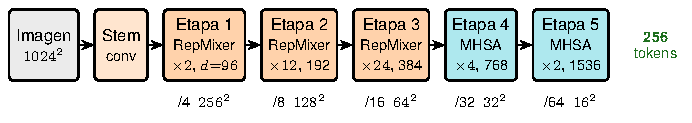
\includegraphics[width=\textwidth]{Figuras/fastvithd_etapas}
  \vspace{3mm}
  \begin{columns}[T]
    \column{.5\textwidth}
    \small
    \begin{itemize}
      \item \textbf{5 etapas}: RepMixer en 1–3, autoatención multi-cabeza en 4–5. Profundidades $[2,12,24,4,2]$; dims. $[96,\dots,1536]$.
      \item \textbf{RepMixer} (de FastViT): mezcla de tokens con conv depthwise; en inferencia sus ramas se \alert{reparametrizan} en una sola conv, sin salto residual $\Rightarrow$ menos accesos a memoria.
      \item \alert{125.1M} parámetros, menos que ViT-L/14 (304M) o SigLIP-SO400M (430M).
    \end{itemize}
    \column{.5\textwidth}
    \small
    \begin{itemize}
      \item Escalar el híbrido de forma ingenua (más atención en las etapas 3–4) es \alert{subóptimo}, incluso más lento que ConvNeXt-L.
      \item Clave: etapa extra con downsampling $\Rightarrow$ la atención opera a \alert{/32} (no /16 como ViTamin) y la salida a /64.
      \item Preentrenado tipo MobileCLIP en \textbf{DataCompDR-1B}.
    \end{itemize}
  \end{columns}
  \refbox{FastVLM, §3.2 y Fig.~2 (resoluciones calculadas para entrada de $1024^2$)}
\end{frame}



\begin{frame}{Resolución, tokens y latencia: FastViTHD vs. ConvNeXt}
  \begin{columns}[c]
    \column{.58\textwidth}
    \centering\scriptsize
    \begin{tabular}{llrrrr}
      \toprule
      Encoder & Res. & Lat. (ms) & Tokens & TextVQA & Avg-5 \\
      \midrule
      \textbf{FastViTHD} & 256 & 10.1 & 16 & 53.1 & 55.5 \\
      ConvNeXt-L & 320 & 34.4 & 100 & 55.5 & 57.7 \\
      ConvNeXt-XXL & 256 & 89.9 & 64 & 56.3 & 58.3 \\
      \textbf{FastViTHD} & 512 & 33.5 & 64 & 59.3 & 60.4 \\
      \midrule
      \textbf{FastViTHD} & 768 & 122.6 & 144 & 62.9 & 62.8 \\
      ConvNeXt-L & 512 & 71.9 & 256 & 61.0 & 61.3 \\
      ConvNeXt-XXL & 512 & 397.1 & 256 & 65.1 & 63.9 \\
      \textbf{FastViTHD} & 1024 & 235.6 & 256 & 64.4 & 63.9 \\
      \bottomrule
    \end{tabular}
    \column{.42\textwidth}
    \centering
    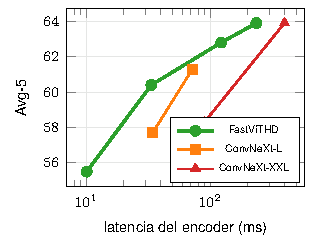
\includegraphics[width=\linewidth]{Figuras/fastvithd_pareto}
  \end{columns}
  \vspace{2mm}
  \small FastViTHD iguala a ConvNeXt-XXL (Avg-5 63.9) siendo \alert{6.8$\times$ más pequeño} y \alert{3.3$\times$ más rápido}. Frente a ViT-L/14 en zero-shot CLIP (38 tareas): rendimiento comparable, 2.4$\times$ más pequeño y 6.9$\times$ más rápido.
  \refbox{FastVLM, Tablas 3–4 (LLaVA-1.5, Vicuna-7B; latencias en M1 MacBook Pro)}
\end{frame}

\begin{frame}{Interacción encoder–LLM: la frontera de Pareto}
  \begin{columns}[T]
    \column{.5\textwidth}
    \small
    \textbf{Pregunta:} con un presupuesto de TTFT, ¿qué combinación de (resolución, tamaño de LLM) da la mejor precisión?
    \begin{itemize}
      \item Barrido: Qwen2 0.5B/1.5B/7B $\times$ varias resoluciones.
      \item Con FastViTHD la frontera de Pareto mejora \alert{$>$2.5 puntos} de Avg-5 sobre FastViT, o alcanza la misma precisión hasta \alert{3$\times$ más rápido}.
      \item A alta resolución, la latencia del \alert{encoder domina} el TTFT.
      \item Un LLM grande a baja resolución suele ser peor que uno más chico con más resolución.
    \end{itemize}
    \column{.5\textwidth}
    \small
    \textbf{Resolución estática vs. dinámica (tiling)}
    \begin{itemize}
      \item Para FastViTHD, fijar directamente la resolución del encoder da el mejor compromiso.
      \item El tiling (AnyRes) sólo ayuda en extremos como $1536^2$, por límites de ancho de banda de memoria.
      \item Si se usa tiling, \alert{menos mosaicos} es mejor.
    \end{itemize}
    \begin{exampleblock}{Mensaje}
      \small Hay que diseñar el encoder \alert{pensando en el TTFT completo}, no sólo en sus FLOPs.
    \end{exampleblock}
  \end{columns}
  \refbox{FastVLM, §3.2.1–§3.2.2, Figs.~4–6}
\end{frame}

\begin{frame}{¿Encoder jerárquico o poda de tokens?}
  \centering\scriptsize
  \begin{tabular}{l r r rrrrrr}
    \toprule
    Método & Res. & Tokens & GQA & SQA & TextVQA & POPE & VQAv2 & SeedB.\\
    \midrule
    ViT-L/14 + MQT & 336 & 16 & 57.6 & 67.5 & -- & 80.8 & 71.1 & --\\
    \textbf{FastViTHD} & 256 & 16 & \textbf{60.6} & \textbf{69.2} & 53.1 & \textbf{82.3} & \textbf{74.7} & 58.8\\
    \midrule
    ViT-L/14 + VisionZip & 336 & 64 & 55.1 & \textbf{69.0} & 55.5 & 77.0 & 62.9 & 52.2\\
    ViT-L/14 + SparseVLM & 336 & 64 & 52.7 & 62.2 & 51.8 & 75.1 & 68.2 & 51.1\\
    \textbf{FastViTHD} & 512 & 64 & \textbf{63.0} & 68.9 & \textbf{59.3} & \textbf{86.4} & \textbf{78.0} & \textbf{61.8}\\
    \midrule
    ViT-L/14 + VisionZip & 336 & 192 & 59.3 & \textbf{68.9} & 57.3 & 85.3 & 76.8 & 56.4\\
    \textbf{FastViTHD} & 768 & 144 & \textbf{62.4} & 67.6 & \textbf{62.9} & \textbf{87.7} & \textbf{78.9} & \textbf{62.5}\\
    \bottomrule
  \end{tabular}
  \vspace{4mm}
  \raggedright
  \begin{itemize}\small
    \item Bajar la \alert{resolución de entrada} de un encoder jerárquico supera a podar tokens de un ViT isotrópico (FastViTHD con 144 tokens supera a VisionZip con 192).
    \item Diseño más simple: sin módulos de poda ni remuestreadores.
  \end{itemize}
  \refbox{FastVLM, §3.2.3 y Tabla 5 (selección de filas; LLaVA-1.5, Vicuna-7B)}
\end{frame}

\begin{frame}{FastVLM: entrenamiento y resultados}
  \begin{columns}[T]
    \column{.45\textwidth}
    \small
    \textbf{Etapas de entrenamiento}
    \begin{enumerate}
      \item \textbf{Etapa 1}: sólo el proyector (LLaVA-558K), a la resolución de preentrenamiento del encoder.
      \item \textbf{Etapa 1.5}: escalado de resolución (15M muestras).
      \item \textbf{Etapa 2}: instrucción visual; se entrena \alert{todo} (encoder, proyector, LLM).
      \item (Etapa 3: ajuste con datos de razonamiento paso a paso.)
    \end{enumerate}
    \scriptsize En un nodo con 8$\times$H100: a $1024^2$, etapa 1.5 $\approx$ 77 h y etapa 2 $\approx$ 8 h.
    \column{.55\textwidth}
    \small
    \textbf{Resultados destacados}
    \begin{itemize}
      \item LLaVA-1.5: \alert{3.2$\times$} mejor TTFT que con SigLIP-SO400M, con encoder 3.6$\times$ más pequeño.
      \item Contra LLaVA-OneVision a $1152^2$ (0.5B LLM): mejor en SeedBench, MMMU y DocVQA con TTFT \alert{85$\times$ menor} (166 ms vs. 14\,124 ms) y encoder 3.4$\times$ más pequeño.
      \item Contra ConvLLaVA (mismo LLM y datos similares): +8.4\% TextVQA, +12.5\% DocVQA, 22\% más rápido.
      \item Con 15M+12.5M muestras supera a MM1 y LLaVA-NeXT generando \alert{5$\times$ menos} tokens que MM1.
    \end{itemize}
  \end{columns}
  \refbox{FastVLM, §4, Tabla 6 (TTFT medido en M1 MacBook Pro)}
\end{frame}

% ============================================================
\section{Síntesis}
% ============================================================

\begin{frame}{Comparación de los trabajos}
  \centering\scriptsize
  \renewcommand{\arraystretch}{1.2}\setlength{\tabcolsep}{3pt}
  \resizebox{\textwidth}{!}{%
  \begin{tabular}{>{\raggedright\arraybackslash}p{1.6cm} >{\raggedright\arraybackslash}p{2.2cm} >{\raggedright\arraybackslash}p{2.3cm} >{\raggedright\arraybackslash}p{2.5cm} >{\raggedright\arraybackslash}p{2.3cm} >{\raggedright\arraybackslash}p{2.7cm}}
    \toprule
    & \textbf{ViT} & \textbf{CLIP} & \textbf{COMM} & \textbf{FasterViT} & \textbf{FastVLM / FastViTHD} \\
    \midrule
    Aporte & Transformer sobre parches & Objetivo contrastivo imagen–texto & Qué encoder y qué capa usar; fusión CLIP + DINOv2 & Híbrido + atención jerárquica (HAT) & Encoder híbrido para VLM + análisis de TTFT \\
    Tipo & Isotrópico & Doble torre (ResNet/ViT + texto) & Dos ViT-L isotrópicos & Jerárquico, 4 etapas & Jerárquico, 5 etapas \\
    Mezcla de tokens & Atención global & (según encoder) & Atención global & Conv $\to$ HAT & RepMixer $\to$ MHSA \\
    Costo vs.\ $N$ & $\mathcal{O}(N^2)$ & (según encoder) & $2\times$ ViT, $\mathcal{O}(N^2)$ & $\approx$ lineal & conv lineal; atención a /32 \\
    Preentren. & Supervisado (JFT, IN-21k) & 400M pares WIT & CLIP + DINOv2 (congelados) & Supervisado (IN-1k/21k) & CLIP en DataCompDR-1B \\
    Uso de capas & Última ([CLS]) & Embedding final & \alert{Todas las capas}, ponderadas & Última etapa & \alert{Varias etapas} (DWConv) \\
    Rol en VLMs & Columna vertebral & Alineación con lenguaje & Percepción fina, grounding & Atención eficiente & Alta resolución con pocos tokens \\
    \bottomrule
  \end{tabular}}
  \vspace{1mm}

  \scriptsize Marco general (survey): todos estos son encoders de las eras 1–2; en las eras nativas la fusión ocurre antes, pero sigue habiendo un encoder o tokenizador visual.
\end{frame}

\begin{frame}{Ideas para llevarse}
  \begin{enumerate}\small
    \item La arquitectura de los VLMs \alert{evolucionó por eras} (dos torres $\to$ LLM + adaptador $\to$ fusión nativa); el encoder visual sigue presente en todas.
    \item \textbf{ViT} convirtió la imagen en una secuencia de tokens; eso la hace ``digerible'' por un LLM.
    \item \textbf{CLIP} le dio a esos tokens \alert{semántica lingüística} a escala Internet; por eso casi todo VLM parte de un encoder CLIP-like.
    \item \textbf{COMM}: la supervisión de CLIP es global. Las \alert{capas superficiales} y los encoders autosupervisados (\alert{DINOv2}) aportan detalle fino; combinarlos mejora el grounding.
    \item El cuello de botella actual es la \alert{resolución}: $N_v\propto r^2$ y la atención es cuadrática en $N_v$.
    \item Los encoders \textbf{jerárquicos / híbridos} reducen tokens \emph{por diseño}; \textbf{FasterViT} logra atención global barata con \emph{carrier tokens}.
    \item \textbf{FastVLM}: optimizar la \alert{latencia de punta a punta} (TTFT); escalar resolución vale más que podar tokens.
  \end{enumerate}
\end{frame}

\begin{frame}{Preguntas para discusión}
  \begin{enumerate}\small
    \item ViT necesita mucho más datos que una CNN. ¿Por qué esa desventaja casi desaparece cuando el encoder se preentrena con CLIP?
    \item En la pérdida InfoNCE, ¿qué papel juega el tamaño del batch? ¿Qué pasa si $\tau\to0$ o $\tau\to\infty$?
    \item Comparen \emph{carrier tokens} (FasterViT) con el token \texttt{[CLS]} de ViT y con las queries de un Q-Former. ¿Qué tienen en común?
    \item FastViTHD hace la atención a /32. Si el VLM tiene que leer texto pequeño en un documento, ¿qué riesgo trae un stride de salida de 64? ¿Cómo ayudan los features multiescala?
    \item Escriban el TTFT como función de $r$ para ViT-L/14 y para FastViTHD, suponiendo $T_{\text{prefill}}$ lineal en tokens. ¿A partir de qué $r$ domina el encoder?
    \item ¿Tiene sentido preentrenar FasterViT con CLIP y usarlo en un VLM? ¿Qué cambiaría respecto a FastViTHD?
    \item COMM muestra que DINOv2, \emph{sin texto}, funciona como rama visual con sólo un MLP, mientras que DeiT supervisado no. ¿Qué dice eso sobre lo que realmente necesita el proyector?
  \end{enumerate}
\end{frame}


\begin{frame}{Lecturas de la clase}
	\small
	\begin{enumerate}
		\item \textbf{ViT} — Dosovitskiy et al., ICLR 2021. \texttt{arXiv:2010.11929}
		\item \textbf{CLIP} — Radford et al., ICML 2021. \texttt{arXiv:2103.00020}
		\item \textbf{COMM} — Jiang et al., \emph{From CLIP to DINO: Visual Encoders Shout in MLLMs}. \texttt{arXiv:2310.08825}
		\item \textbf{FasterViT} — Hatamizadeh et al. (NVIDIA), ICLR 2024. \texttt{arXiv:2306.06189}
		\item \textbf{FastVLM} — Vasu et al. (Apple), CVPR 2025. \texttt{arXiv:2412.13303}
		\item \textbf{Survey} — Li et al., \emph{Frontier VLMs: Architectural Evolution, Benchmarks, Applications, and Challenges}. \texttt{arXiv:2501.02189}
	\end{enumerate}
	\vspace{2mm}
	\begin{alertblock}{Ojo con los nombres}
		\textbf{FasterViT} (NVIDIA, atención jerárquica) $\neq$ \textbf{FastViT} (Apple, RepMixer, base de FastVLM).
	\end{alertblock}
\end{frame}


\begin{frame}{Referencias}
  \scriptsize
  \begin{enumerate}\setlength{\itemsep}{1.5pt}
    \item A.~Dosovitskiy, L.~Beyer, A.~Kolesnikov, D.~Weissenborn, X.~Zhai, T.~Unterthiner, M.~Dehghani, M.~Minderer, G.~Heigold, S.~Gelly, J.~Uszkoreit, N.~Houlsby. \emph{An Image is Worth 16x16 Words: Transformers for Image Recognition at Scale}. ICLR, 2021. arXiv:2010.11929.
    \item A.~Radford, J.~W.~Kim, C.~Hallacy, A.~Ramesh, G.~Goh, S.~Agarwal, G.~Sastry, A.~Askell, P.~Mishkin, J.~Clark, G.~Krueger, I.~Sutskever. \emph{Learning Transferable Visual Models From Natural Language Supervision}. ICML, 2021. arXiv:2103.00020.
    \item D.~Jiang, Y.~Liu, S.~Liu, J.~Zhao, H.~Zhang, Z.~Gao, X.~Zhang, J.~Li, H.~Xiong. \emph{From CLIP to DINO: Visual Encoders Shout in Multi-modal Large Language Models}. arXiv:2310.08825, 2023.
    \item Z.~Li, X.~Wu, H.~Du, F.~Liu, H.~Nghiem, G.~Shi. \emph{Frontier Vision-Language Models: Architectural Evolution, Benchmarks, Applications, and Challenges}. arXiv:2501.02189 (v7), 2026.
    \item A.~Hatamizadeh, G.~Heinrich, H.~Yin, A.~Tao, J.~M.~Alvarez, J.~Kautz, P.~Molchanov. \emph{FasterViT: Fast Vision Transformers with Hierarchical Attention}. ICLR, 2024. arXiv:2306.06189.
    \item P.~K.~A.~Vasu, F.~Faghri, C.-L.~Li, C.~Koc, N.~True, A.~Antony, G.~Santhanam, J.~Gabriel, P.~Grasch, O.~Tuzel, H.~Pouransari. \emph{FastVLM: Efficient Vision Encoding for Vision Language Models}. CVPR, 2025. arXiv:2412.13303.
    \item P.~K.~A.~Vasu, J.~Gabriel, J.~Zhu, O.~Tuzel, A.~Ranjan. \emph{FastViT: A Fast Hybrid Vision Transformer using Structural Reparameterization}. ICCV, 2023. (Citada en FastVLM.)
    \item H.~Liu, C.~Li, Q.~Wu, Y.~J.~Lee. \emph{Visual Instruction Tuning} (LLaVA). NeurIPS, 2023. arXiv:2304.08485.
    \item H.~Liu, C.~Li, Y.~Li, Y.~J.~Lee. \emph{Improved Baselines with Visual Instruction Tuning} (LLaVA-1.5). CVPR, 2024. arXiv:2310.03744.
  \end{enumerate}
\end{frame}

\begin{frame}[standout]
	Preguntas
\end{frame}

\end{document}
